\documentclass[tikz,border=5pt]{standalone}
\begin{document}
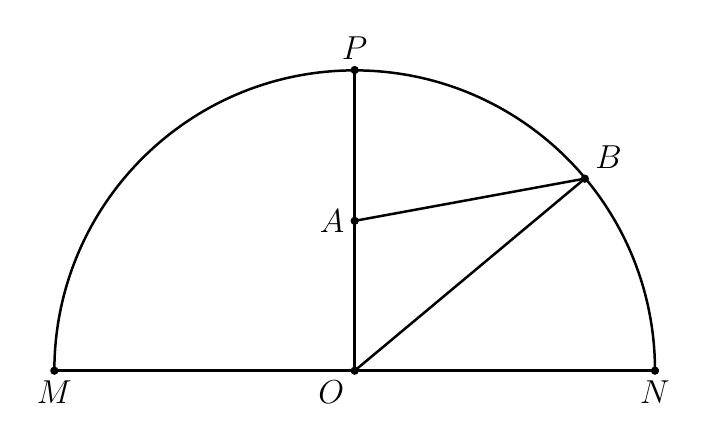
\begin{tikzpicture}[line join=round, line width=0.9pt]
  % Coordinates (cm): s = 0.016064 cm/px, y-axis flipped, origin at O
  \coordinate (O) at (0,-1.885);
  \coordinate (M) at (-3.814,-1.885);   % left end of diameter
  \coordinate (N) at (3.814,-1.885);    % right end of diameter
  \coordinate (P) at (0,1.933);         % top of vertical radius
  \coordinate (A) at (0,0.018);         % point on OP
  \coordinate (B) at (2.923,0.554);     % point on the arc

  % Diameter MN
  \draw (M) -- (N);

  % Upper semicircle centred at O, radius 3.814 (M to N through top)
  \draw (M) arc[start angle=180, end angle=0, radius=3.814];

  % Vertical radius O to P
  \draw (O) -- (P);

  % Segments B-O and B-A
  \draw (B) -- (O);
  \draw (B) -- (A);

  % Small filled dots at points
  \foreach \X in {O,M,N,P,A,B}
    \fill (\X) circle (1.5pt);

  % Labels
  \node[font=\fontsize{12.5}{15}\selectfont, above] at (P) {$P$};
  \node[font=\fontsize{12.5}{15}\selectfont, left] at (A) {$A$};
  \node[font=\fontsize{12.5}{15}\selectfont, above right] at (B) {$B$};
  \node[font=\fontsize{12.5}{15}\selectfont, below left] at (O) {$O$};
  \node[font=\fontsize{12.5}{15}\selectfont, below] at (M) {$M$};
  \node[font=\fontsize{12.5}{15}\selectfont, below] at (N) {$N$};
\end{tikzpicture}
\end{document}